% SOURCE: ../../edit-harness/results/D3_benefit_predictor_eval.json
% !TEX encoding = UTF-8 Unicode
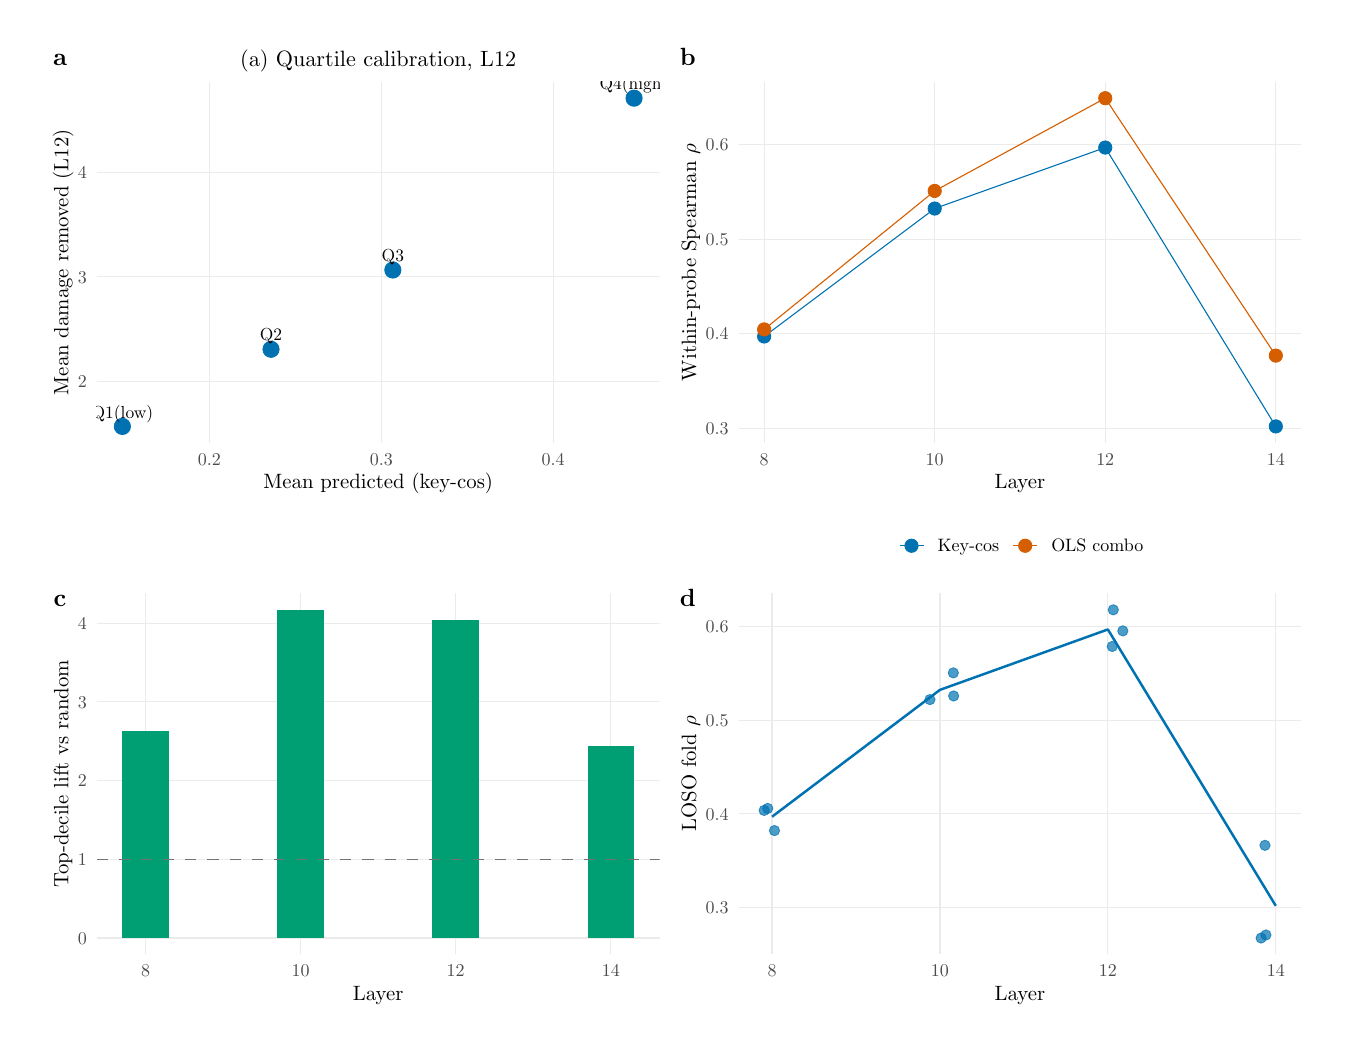
\begin{tikzpicture}[x=1pt,y=1pt]
\definecolor{fillColor}{RGB}{255,255,255}
\path[use as bounding box,fill=fillColor,fill opacity=0.00] (0,0) rectangle (469.75,361.35);
\begin{scope}
\path[clip] (  0.00,  0.00) rectangle (469.75,361.35);
\definecolor{drawColor}{RGB}{255,255,255}
\definecolor{fillColor}{RGB}{255,255,255}

\path[draw=drawColor,line width= 0.6pt,line join=round,line cap=round,fill=fillColor] (  0.00,  0.00) rectangle (469.76,361.35);
\end{scope}
\begin{scope}
\path[clip] (  5.50,159.92) rectangle (232.35,355.85);
\definecolor{fillColor}{RGB}{255,255,255}

\path[fill=fillColor] (  5.50,159.92) rectangle (232.35,355.85);
\end{scope}
\begin{scope}
\path[clip] (232.35,159.92) rectangle (464.26,355.85);
\definecolor{fillColor}{RGB}{255,255,255}

\path[fill=fillColor] (232.35,159.92) rectangle (464.25,355.85);
\end{scope}
\begin{scope}
\path[clip] (  5.50,  5.50) rectangle (232.35,159.92);
\definecolor{fillColor}{RGB}{255,255,255}

\path[fill=fillColor] (  5.50,  5.50) rectangle (232.35,159.92);
\end{scope}
\begin{scope}
\path[clip] (232.35,  5.50) rectangle (464.26,159.92);
\definecolor{fillColor}{RGB}{255,255,255}

\path[fill=fillColor] (232.35,  5.50) rectangle (464.25,159.92);
\end{scope}
\begin{scope}
\path[clip] ( 24.97,211.33) rectangle (228.35,341.79);
\definecolor{drawColor}{gray}{0.92}

\path[draw=drawColor,line width= 0.4pt,line join=round] ( 24.97,233.47) --
	(228.35,233.47);

\path[draw=drawColor,line width= 0.4pt,line join=round] ( 24.97,271.31) --
	(228.35,271.31);

\path[draw=drawColor,line width= 0.4pt,line join=round] ( 24.97,309.15) --
	(228.35,309.15);

\path[draw=drawColor,line width= 0.4pt,line join=round] ( 65.69,211.33) --
	( 65.69,341.79);

\path[draw=drawColor,line width= 0.4pt,line join=round] (127.77,211.33) --
	(127.77,341.79);

\path[draw=drawColor,line width= 0.4pt,line join=round] (189.85,211.33) --
	(189.85,341.79);
\definecolor{drawColor}{RGB}{0,114,178}
\definecolor{fillColor}{RGB}{0,114,178}

\path[draw=drawColor,line width= 0.3pt,line join=round,line cap=round,fill=fillColor] ( 34.22,217.26) circle (  2.94);

\path[draw=drawColor,line width= 0.3pt,line join=round,line cap=round,fill=fillColor] ( 87.93,245.13) circle (  2.94);

\path[draw=drawColor,line width= 0.3pt,line join=round,line cap=round,fill=fillColor] (131.95,273.78) circle (  2.94);

\path[draw=drawColor,line width= 0.3pt,line join=round,line cap=round,fill=fillColor] (219.11,335.86) circle (  2.94);
\definecolor{drawColor}{RGB}{0,0,0}

\node[text=drawColor,anchor=base,inner sep=0pt, outer sep=0pt, scale=  0.63] at ( 34.22,220.28) {Q1(low)};

\node[text=drawColor,anchor=base,inner sep=0pt, outer sep=0pt, scale=  0.63] at ( 87.93,248.15) {Q2};

\node[text=drawColor,anchor=base,inner sep=0pt, outer sep=0pt, scale=  0.63] at (131.95,276.79) {Q3};

\node[text=drawColor,anchor=base,inner sep=0pt, outer sep=0pt, scale=  0.63] at (219.11,338.87) {Q4(high)};
\definecolor{drawColor}{gray}{0.50}

\path[draw=drawColor,line width= 0.5pt,dash pattern=on 4pt off 4pt ,line join=round] (-178.41,150.47) -- (431.73,187.66);
\end{scope}
\begin{scope}
\path[clip] (  0.00,  0.00) rectangle (469.75,361.35);
\definecolor{drawColor}{gray}{0.30}

\node[text=drawColor,anchor=base east,inner sep=0pt, outer sep=0pt, scale=  0.65] at ( 21.37,231.23) {2};

\node[text=drawColor,anchor=base east,inner sep=0pt, outer sep=0pt, scale=  0.65] at ( 21.37,269.07) {3};

\node[text=drawColor,anchor=base east,inner sep=0pt, outer sep=0pt, scale=  0.65] at ( 21.37,306.91) {4};
\end{scope}
\begin{scope}
\path[clip] (  0.00,  0.00) rectangle (469.75,361.35);
\definecolor{drawColor}{gray}{0.30}

\node[text=drawColor,anchor=base,inner sep=0pt, outer sep=0pt, scale=  0.65] at ( 65.69,203.26) {0.2};

\node[text=drawColor,anchor=base,inner sep=0pt, outer sep=0pt, scale=  0.65] at (127.77,203.26) {0.3};

\node[text=drawColor,anchor=base,inner sep=0pt, outer sep=0pt, scale=  0.65] at (189.85,203.26) {0.4};
\end{scope}
\begin{scope}
\path[clip] (  0.00,  0.00) rectangle (469.75,361.35);
\definecolor{drawColor}{RGB}{0,0,0}

\node[text=drawColor,anchor=base,inner sep=0pt, outer sep=0pt, scale=  0.75] at (126.66,194.83) {Mean predicted (key-cos)};
\end{scope}
\begin{scope}
\path[clip] (  0.00,  0.00) rectangle (469.75,361.35);
\definecolor{drawColor}{RGB}{0,0,0}

\node[text=drawColor,rotate= 90.00,anchor=base,inner sep=0pt, outer sep=0pt, scale=  0.75] at ( 14.67,276.56) {Mean damage removed (L12)};
\end{scope}
\begin{scope}
\path[clip] (  0.00,  0.00) rectangle (469.75,361.35);
\definecolor{drawColor}{RGB}{0,0,0}

\node[text=drawColor,anchor=base,inner sep=0pt, outer sep=0pt, scale=  0.80] at (126.66,347.34) {(a) Quartile calibration, L12};
\end{scope}
\begin{scope}
\path[clip] (  0.00,  0.00) rectangle (469.75,361.35);
\definecolor{drawColor}{RGB}{0,0,0}

\node[text=drawColor,anchor=base,inner sep=0pt, outer sep=0pt, scale=  0.90] at ( 11.69,347.85) {\bfseries a};
\end{scope}
\begin{scope}
\path[clip] (256.88,211.33) rectangle (460.25,341.79);
\definecolor{drawColor}{gray}{0.92}

\path[draw=drawColor,line width= 0.4pt,line join=round] (256.88,216.65) --
	(460.25,216.65);

\path[draw=drawColor,line width= 0.4pt,line join=round] (256.88,250.80) --
	(460.25,250.80);

\path[draw=drawColor,line width= 0.4pt,line join=round] (256.88,284.96) --
	(460.25,284.96);

\path[draw=drawColor,line width= 0.4pt,line join=round] (256.88,319.12) --
	(460.25,319.12);

\path[draw=drawColor,line width= 0.4pt,line join=round] (266.12,211.33) --
	(266.12,341.79);

\path[draw=drawColor,line width= 0.4pt,line join=round] (327.75,211.33) --
	(327.75,341.79);

\path[draw=drawColor,line width= 0.4pt,line join=round] (389.38,211.33) --
	(389.38,341.79);

\path[draw=drawColor,line width= 0.4pt,line join=round] (451.01,211.33) --
	(451.01,341.79);
\definecolor{drawColor}{RGB}{0,114,178}

\path[draw=drawColor,line width= 0.4pt,line join=round] (266.12,249.75) --
	(327.75,295.99) --
	(389.38,318.03) --
	(451.01,217.26);
\definecolor{drawColor}{RGB}{213,94,0}

\path[draw=drawColor,line width= 0.4pt,line join=round] (266.12,252.31) --
	(327.75,302.35) --
	(389.38,335.86) --
	(451.01,242.85);
\definecolor{drawColor}{RGB}{0,114,178}
\definecolor{fillColor}{RGB}{0,114,178}

\path[draw=drawColor,line width= 0.3pt,line join=round,line cap=round,fill=fillColor] (266.12,249.75) circle (  2.40);

\path[draw=drawColor,line width= 0.3pt,line join=round,line cap=round,fill=fillColor] (327.75,295.99) circle (  2.40);

\path[draw=drawColor,line width= 0.3pt,line join=round,line cap=round,fill=fillColor] (389.38,318.03) circle (  2.40);

\path[draw=drawColor,line width= 0.3pt,line join=round,line cap=round,fill=fillColor] (451.01,217.26) circle (  2.40);
\definecolor{drawColor}{RGB}{213,94,0}
\definecolor{fillColor}{RGB}{213,94,0}

\path[draw=drawColor,line width= 0.3pt,line join=round,line cap=round,fill=fillColor] (266.12,252.31) circle (  2.40);

\path[draw=drawColor,line width= 0.3pt,line join=round,line cap=round,fill=fillColor] (327.75,302.35) circle (  2.40);

\path[draw=drawColor,line width= 0.3pt,line join=round,line cap=round,fill=fillColor] (389.38,335.86) circle (  2.40);

\path[draw=drawColor,line width= 0.3pt,line join=round,line cap=round,fill=fillColor] (451.01,242.85) circle (  2.40);
\end{scope}
\begin{scope}
\path[clip] (  0.00,  0.00) rectangle (469.75,361.35);
\definecolor{drawColor}{gray}{0.30}

\node[text=drawColor,anchor=base east,inner sep=0pt, outer sep=0pt, scale=  0.65] at (253.28,214.41) {0.3};

\node[text=drawColor,anchor=base east,inner sep=0pt, outer sep=0pt, scale=  0.65] at (253.28,248.57) {0.4};

\node[text=drawColor,anchor=base east,inner sep=0pt, outer sep=0pt, scale=  0.65] at (253.28,282.72) {0.5};

\node[text=drawColor,anchor=base east,inner sep=0pt, outer sep=0pt, scale=  0.65] at (253.28,316.88) {0.6};
\end{scope}
\begin{scope}
\path[clip] (  0.00,  0.00) rectangle (469.75,361.35);
\definecolor{drawColor}{gray}{0.30}

\node[text=drawColor,anchor=base,inner sep=0pt, outer sep=0pt, scale=  0.65] at (266.12,203.26) {8};

\node[text=drawColor,anchor=base,inner sep=0pt, outer sep=0pt, scale=  0.65] at (327.75,203.26) {10};

\node[text=drawColor,anchor=base,inner sep=0pt, outer sep=0pt, scale=  0.65] at (389.38,203.26) {12};

\node[text=drawColor,anchor=base,inner sep=0pt, outer sep=0pt, scale=  0.65] at (451.01,203.26) {14};
\end{scope}
\begin{scope}
\path[clip] (  0.00,  0.00) rectangle (469.75,361.35);
\definecolor{drawColor}{RGB}{0,0,0}

\node[text=drawColor,anchor=base,inner sep=0pt, outer sep=0pt, scale=  0.75] at (358.57,194.83) {Layer};
\end{scope}
\begin{scope}
\path[clip] (  0.00,  0.00) rectangle (469.75,361.35);
\definecolor{drawColor}{RGB}{0,0,0}

\node[text=drawColor,rotate= 90.00,anchor=base,inner sep=0pt, outer sep=0pt, scale=  0.75] at (241.52,276.56) {Within-probe Spearman $\rho$};
\end{scope}
\begin{scope}
\path[clip] (  0.00,  0.00) rectangle (469.75,361.35);
\definecolor{drawColor}{RGB}{0,114,178}

\path[draw=drawColor,line width= 0.4pt,line join=round] (315.04,174.14) -- (323.71,174.14);
\definecolor{fillColor}{RGB}{0,114,178}

\path[draw=drawColor,line width= 0.3pt,line join=round,line cap=round,fill=fillColor] (319.37,174.14) circle (  2.40);
\end{scope}
\begin{scope}
\path[clip] (  0.00,  0.00) rectangle (469.75,361.35);
\definecolor{drawColor}{RGB}{213,94,0}

\path[draw=drawColor,line width= 0.4pt,line join=round] (356.12,174.14) -- (364.79,174.14);
\definecolor{fillColor}{RGB}{213,94,0}

\path[draw=drawColor,line width= 0.3pt,line join=round,line cap=round,fill=fillColor] (360.45,174.14) circle (  2.40);
\end{scope}
\begin{scope}
\path[clip] (  0.00,  0.00) rectangle (469.75,361.35);
\definecolor{drawColor}{RGB}{0,0,0}

\node[text=drawColor,anchor=base west,inner sep=0pt, outer sep=0pt, scale=  0.65] at (328.79,171.90) {Key-cos};
\end{scope}
\begin{scope}
\path[clip] (  0.00,  0.00) rectangle (469.75,361.35);
\definecolor{drawColor}{RGB}{0,0,0}

\node[text=drawColor,anchor=base west,inner sep=0pt, outer sep=0pt, scale=  0.65] at (369.87,171.90) {OLS combo};
\end{scope}
\begin{scope}
\path[clip] (  0.00,  0.00) rectangle (469.75,361.35);
\definecolor{drawColor}{RGB}{0,0,0}

\node[text=drawColor,anchor=base,inner sep=0pt, outer sep=0pt, scale=  0.90] at (238.59,347.85) {\bfseries b};
\end{scope}
\begin{scope}
\path[clip] ( 24.97, 26.46) rectangle (228.35,156.92);
\definecolor{drawColor}{gray}{0.92}

\path[draw=drawColor,line width= 0.4pt,line join=round] ( 24.97, 32.39) --
	(228.35, 32.39);

\path[draw=drawColor,line width= 0.4pt,line join=round] ( 24.97, 60.83) --
	(228.35, 60.83);

\path[draw=drawColor,line width= 0.4pt,line join=round] ( 24.97, 89.27) --
	(228.35, 89.27);

\path[draw=drawColor,line width= 0.4pt,line join=round] ( 24.97,117.71) --
	(228.35,117.71);

\path[draw=drawColor,line width= 0.4pt,line join=round] ( 24.97,146.15) --
	(228.35,146.15);

\path[draw=drawColor,line width= 0.4pt,line join=round] ( 42.62, 26.46) --
	( 42.62,156.92);

\path[draw=drawColor,line width= 0.4pt,line join=round] ( 98.65, 26.46) --
	( 98.65,156.92);

\path[draw=drawColor,line width= 0.4pt,line join=round] (154.67, 26.46) --
	(154.67,156.92);

\path[draw=drawColor,line width= 0.4pt,line join=round] (210.70, 26.46) --
	(210.70,156.92);
\definecolor{fillColor}{RGB}{0,158,115}

\path[fill=fillColor] ( 34.22, 32.39) rectangle ( 51.03,107.19);

\path[fill=fillColor] ( 90.24, 32.39) rectangle (107.05,150.99);

\path[fill=fillColor] (146.27, 32.39) rectangle (163.08,147.29);

\path[fill=fillColor] (202.30, 32.39) rectangle (219.11,101.79);
\definecolor{drawColor}{gray}{0.45}

\path[draw=drawColor,line width= 0.3pt,dash pattern=on 4pt off 4pt ,line join=round] ( 24.97, 60.83) -- (228.35, 60.83);
\end{scope}
\begin{scope}
\path[clip] (  0.00,  0.00) rectangle (469.75,361.35);
\definecolor{drawColor}{gray}{0.30}

\node[text=drawColor,anchor=base east,inner sep=0pt, outer sep=0pt, scale=  0.65] at ( 21.37, 30.15) {0};

\node[text=drawColor,anchor=base east,inner sep=0pt, outer sep=0pt, scale=  0.65] at ( 21.37, 58.59) {1};

\node[text=drawColor,anchor=base east,inner sep=0pt, outer sep=0pt, scale=  0.65] at ( 21.37, 87.03) {2};

\node[text=drawColor,anchor=base east,inner sep=0pt, outer sep=0pt, scale=  0.65] at ( 21.37,115.47) {3};

\node[text=drawColor,anchor=base east,inner sep=0pt, outer sep=0pt, scale=  0.65] at ( 21.37,143.91) {4};
\end{scope}
\begin{scope}
\path[clip] (  0.00,  0.00) rectangle (469.75,361.35);
\definecolor{drawColor}{gray}{0.30}

\node[text=drawColor,anchor=base,inner sep=0pt, outer sep=0pt, scale=  0.65] at ( 42.62, 18.39) {8};

\node[text=drawColor,anchor=base,inner sep=0pt, outer sep=0pt, scale=  0.65] at ( 98.65, 18.39) {10};

\node[text=drawColor,anchor=base,inner sep=0pt, outer sep=0pt, scale=  0.65] at (154.67, 18.39) {12};

\node[text=drawColor,anchor=base,inner sep=0pt, outer sep=0pt, scale=  0.65] at (210.70, 18.39) {14};
\end{scope}
\begin{scope}
\path[clip] (  0.00,  0.00) rectangle (469.75,361.35);
\definecolor{drawColor}{RGB}{0,0,0}

\node[text=drawColor,anchor=base,inner sep=0pt, outer sep=0pt, scale=  0.75] at (126.66,  9.96) {Layer};
\end{scope}
\begin{scope}
\path[clip] (  0.00,  0.00) rectangle (469.75,361.35);
\definecolor{drawColor}{RGB}{0,0,0}

\node[text=drawColor,rotate= 90.00,anchor=base,inner sep=0pt, outer sep=0pt, scale=  0.75] at ( 14.67, 91.69) {Top-decile lift vs random};
\end{scope}
\begin{scope}
\path[clip] (  0.00,  0.00) rectangle (469.75,361.35);
\definecolor{drawColor}{RGB}{0,0,0}

\node[text=drawColor,anchor=base,inner sep=0pt, outer sep=0pt, scale=  0.90] at ( 11.69,152.33) {\bfseries c};
\end{scope}
\begin{scope}
\path[clip] (256.88, 26.46) rectangle (460.25,156.92);
\definecolor{drawColor}{gray}{0.92}

\path[draw=drawColor,line width= 0.4pt,line join=round] (256.88, 43.41) --
	(460.25, 43.41);

\path[draw=drawColor,line width= 0.4pt,line join=round] (256.88, 77.27) --
	(460.25, 77.27);

\path[draw=drawColor,line width= 0.4pt,line join=round] (256.88,111.13) --
	(460.25,111.13);

\path[draw=drawColor,line width= 0.4pt,line join=round] (256.88,144.98) --
	(460.25,144.98);

\path[draw=drawColor,line width= 0.4pt,line join=round] (268.97, 26.46) --
	(268.97,156.92);

\path[draw=drawColor,line width= 0.4pt,line join=round] (329.65, 26.46) --
	(329.65,156.92);

\path[draw=drawColor,line width= 0.4pt,line join=round] (390.33, 26.46) --
	(390.33,156.92);

\path[draw=drawColor,line width= 0.4pt,line join=round] (451.01, 26.46) --
	(451.01,156.92);
\definecolor{drawColor}{RGB}{0,114,178}
\definecolor{fillColor}{RGB}{0,114,178}

\path[draw=drawColor,draw opacity=0.70,line width= 0.3pt,line join=round,line cap=round,fill=fillColor,fill opacity=0.70] (266.12, 78.51) circle (  1.87);

\path[draw=drawColor,draw opacity=0.70,line width= 0.3pt,line join=round,line cap=round,fill=fillColor,fill opacity=0.70] (267.42, 79.23) circle (  1.87);

\path[draw=drawColor,draw opacity=0.70,line width= 0.3pt,line join=round,line cap=round,fill=fillColor,fill opacity=0.70] (269.85, 71.22) circle (  1.87);

\path[draw=drawColor,draw opacity=0.70,line width= 0.3pt,line join=round,line cap=round,fill=fillColor,fill opacity=0.70] (334.60,119.86) circle (  1.87);

\path[draw=drawColor,draw opacity=0.70,line width= 0.3pt,line join=round,line cap=round,fill=fillColor,fill opacity=0.70] (326.03,118.55) circle (  1.87);

\path[draw=drawColor,draw opacity=0.70,line width= 0.3pt,line join=round,line cap=round,fill=fillColor,fill opacity=0.70] (334.48,128.20) circle (  1.87);

\path[draw=drawColor,draw opacity=0.70,line width= 0.3pt,line join=round,line cap=round,fill=fillColor,fill opacity=0.70] (395.73,143.38) circle (  1.87);

\path[draw=drawColor,draw opacity=0.70,line width= 0.3pt,line join=round,line cap=round,fill=fillColor,fill opacity=0.70] (392.28,150.99) circle (  1.87);

\path[draw=drawColor,draw opacity=0.70,line width= 0.3pt,line join=round,line cap=round,fill=fillColor,fill opacity=0.70] (391.90,137.75) circle (  1.87);

\path[draw=drawColor,draw opacity=0.70,line width= 0.3pt,line join=round,line cap=round,fill=fillColor,fill opacity=0.70] (445.69, 32.39) circle (  1.87);

\path[draw=drawColor,draw opacity=0.70,line width= 0.3pt,line join=round,line cap=round,fill=fillColor,fill opacity=0.70] (447.44, 33.49) circle (  1.87);

\path[draw=drawColor,draw opacity=0.70,line width= 0.3pt,line join=round,line cap=round,fill=fillColor,fill opacity=0.70] (447.09, 65.89) circle (  1.87);
\definecolor{drawColor}{RGB}{0,114,178}

\path[draw=drawColor,line width= 0.9pt,line join=round] (268.97, 76.22) --
	(268.97, 76.22) --
	(268.97, 76.22) --
	(329.65,122.06) --
	(329.65,122.06) --
	(329.65,122.06) --
	(390.33,143.90) --
	(390.33,143.90) --
	(390.33,143.90) --
	(451.01, 44.02) --
	(451.01, 44.02) --
	(451.01, 44.02);
\end{scope}
\begin{scope}
\path[clip] (  0.00,  0.00) rectangle (469.75,361.35);
\definecolor{drawColor}{gray}{0.30}

\node[text=drawColor,anchor=base east,inner sep=0pt, outer sep=0pt, scale=  0.65] at (253.28, 41.18) {0.3};

\node[text=drawColor,anchor=base east,inner sep=0pt, outer sep=0pt, scale=  0.65] at (253.28, 75.03) {0.4};

\node[text=drawColor,anchor=base east,inner sep=0pt, outer sep=0pt, scale=  0.65] at (253.28,108.89) {0.5};

\node[text=drawColor,anchor=base east,inner sep=0pt, outer sep=0pt, scale=  0.65] at (253.28,142.74) {0.6};
\end{scope}
\begin{scope}
\path[clip] (  0.00,  0.00) rectangle (469.75,361.35);
\definecolor{drawColor}{gray}{0.30}

\node[text=drawColor,anchor=base,inner sep=0pt, outer sep=0pt, scale=  0.65] at (268.97, 18.39) {8};

\node[text=drawColor,anchor=base,inner sep=0pt, outer sep=0pt, scale=  0.65] at (329.65, 18.39) {10};

\node[text=drawColor,anchor=base,inner sep=0pt, outer sep=0pt, scale=  0.65] at (390.33, 18.39) {12};

\node[text=drawColor,anchor=base,inner sep=0pt, outer sep=0pt, scale=  0.65] at (451.01, 18.39) {14};
\end{scope}
\begin{scope}
\path[clip] (  0.00,  0.00) rectangle (469.75,361.35);
\definecolor{drawColor}{RGB}{0,0,0}

\node[text=drawColor,anchor=base,inner sep=0pt, outer sep=0pt, scale=  0.75] at (358.57,  9.96) {Layer};
\end{scope}
\begin{scope}
\path[clip] (  0.00,  0.00) rectangle (469.75,361.35);
\definecolor{drawColor}{RGB}{0,0,0}

\node[text=drawColor,rotate= 90.00,anchor=base,inner sep=0pt, outer sep=0pt, scale=  0.75] at (241.52, 91.69) {LOSO fold $\rho$};
\end{scope}
\begin{scope}
\path[clip] (  0.00,  0.00) rectangle (469.75,361.35);
\definecolor{drawColor}{RGB}{0,0,0}

\node[text=drawColor,anchor=base,inner sep=0pt, outer sep=0pt, scale=  0.90] at (238.59,152.33) {\bfseries d};
\end{scope}
\end{tikzpicture}
